% --------------------------------------------------
% Fájl: main.tex
% --------------------------------------------------

% Dokumentum konfiguráció
\documentclass[12pt]{article}

% --------------------------------------------------
% Dokumentum adatok
% --------------------------------------------------

% Intézmény és kar
\newcommand\INTEZMENY{Budapesti Műszaki és Gazdaságtudományi Egyetem}
\newcommand\KAR{Gépészmérnöki Kar}
\newcommand\LOGO{bme-logo.jpg} % logo fájl neve a figures mappában

% Dokumentum adatok
% TODO
\newcommand\CIM{Egyszerű rakéta szimuláció}
\newcommand\DATUM{2025}
\newcommand\NEV{Illés Gergely Levente}
\newcommand\NEPTUN{EYOXUS}
\newcommand\EMAIL{illesgergelypecs@gmail.com}
\newcommand\TANTARGY{Egyszerű rakéta szimuláció}
\newcommand\TANTARGYKOD{Asztrodinamika}

% --------------------------------------------------
% Preambulum és egyéni parancsok betöltése
% --------------------------------------------------

% \input{settings/00_preambulum.tex}
% --------------------------------------------------
% Fájl: 00_preambulum.tex
% --------------------------------------------------

% --------------------------------------------------
% Packagek
% --------------------------------------------------

% Dokumentum konfiguráció
\usepackage[hungarian]{babel} % dokumentum nyelvi beállítása
\usepackage[utf8]{inputenc} % bemeneti betűkódolás (ékezetes karakterek)
\usepackage[T1]{fontenc} % kimeneti betűkódolás (ékezetes karakterek)
\usepackage{lmodern} % bővített karakterkészlet az ékezetekhez
\usepackage{geometry} % dokumentum margók és oldalbeállítások
\usepackage{hyperref} % hivatkozások és linkek
\usepackage[backend=biber,style=numeric,sorting=none]{biblatex} % irodalomjegyzék
\usepackage{icomma} % 0, 1 helyett 0,1.

% Ábrák, grafikák
\usepackage{graphicx} % klépek beillesztése és méretezése
\usepackage{float} % ábrák és táblázatok elhelyezésének pontos szabályozása
\usepackage{caption} % képaláírások formázása
\usepackage{subcaption}
\usepackage{tikz} % vektorgrafikák, ábrák rajzolása LaTeX-ben
\usepackage{xcolor} % színek kezelése
\usepackage{pdfpages} % teljes PDF-oldalak beillesztése a dokumentumba
\usepackage{calc}
\usepackage{adjustbox}
\usepackage{float} % a [H] opcióhoz
\usepackage{multirow}
\usepackage{hhline}
\usepackage{rotating}
\usepackage{empheq} % szükséges a kapcsos zárójel és számozás kombinálásához

% Matematikai és fizikai írásmód
\usepackage{amsmath,amsthm,amsfonts,amssymb,amscd} % matematikai környezetek és szimbólumok
\usepackage{mathtools} % kiegészítő matematikai eszközök az amsmath-hoz
\usepackage{siunitx} % SI mértékegységek helyes jelölése
\usepackage[scr=rsfs]{mathalpha}
\usepackage{physics}

% Fejléc, lábléc
\usepackage{fancyhdr} % egyedi fejléc és lábléc készítése
\usepackage{lastpage} % az utolsó oldal sorszámának hivatkozása

% Dokumentumtagolás
\usepackage{titlesec} % címsorok formázásának testreszabása
\usepackage{csquotes} % idézetek helyes formázása (nyelvspecifikus)
\usepackage{booktabs} % szép, tipográfiailag helyes táblázatok készítése
\usepackage{placeins} % \FloatBarrier
\usepackage{pdfpages}


\makeatletter
\newcommand{\currentsectionname}{\@currentlabelname}
\makeatother

% --------------------------------------------------
% Dokumentum beállítások
% --------------------------------------------------

% Dokumentum formátum
\geometry{a4paper,total={170mm,240mm},left=20mm,top=30mm} % oldalbeállítások: A4, margók méretezése
\setlength\parindent{0pt} % bekezdések behúzásának kikapcsolása

\sisetup{
  output-decimal-marker = {,}, % vessző a tizedeshez
  group-separator = {\,},      % ezredhelyi elválasztó (opcionális)
  detect-all
}

% Fejléc, lábléc beállítása
\pagestyle{fancy} % fancyhdr csomag stílus használata
\renewcommand{\headrulewidth}{0.4pt} % fejléc vonalvastagsága
\renewcommand{\footrulewidth}{0.4pt} % lábléc vonalvastagsága
\headheight 1.5em % fejléc magasságának beállítása
\rhead{\currentsectionname} % jobb felső sarok
\chead{} % középső fejléc
\lhead{\CIM{}} % bal felső sarok
\lfoot{} % bal alsó sarok
\cfoot{} % középső lábléc
\rfoot{\small\thepage\ / \pageref{LastPage}} % jobb alsó sarok
\headsep 1.5em % fejléc és szöveg közötti távolság

% Hyperref beállítások - PDF megjelenítés
\hypersetup{
    colorlinks=true, % színes linkek
    linkcolor=blue, % belső hivatkozások színe
    urlcolor=teal, % URL hivatkozások színe
    pdftitle={\CIM{}}, % PDF cím
    pdfauthor={\NEV{}}, % PDF szerző
    pdfsubject={\CIM{}}, % PDF tárgy
    bookmarksopen=true, % könyvjelzők alapból nyitva
    bookmarksnumbered=true, % könyvjelzők számozása
    pdfpagemode=UseOutlines % könyvjelzők megjelenítése PDF olvasóban
}

% Irodalomjegyék beállítása
% \addbibresource{contents/literature.bib} % irodalomjegyzék forrásfájl
\addbibresource{figures/asztrodinamika.bib}

% Számozások beállítása fejezetenként
% \numberwithin{equation}{section} % egyenletek számozása fejezetenként
% \numberwithin{figure}{section} % ábrák számozása fejezetenként
% \numberwithin{table}{section} % táblázatok számozása fejezetenként

% Táblázat formátum beállítása - Függőlegesen középre igazított szöveg
\newcolumntype{L}[1]{>{\raggedright\let\newline\\\arraybackslash\hspace{0pt}}m{#1}} % balra zárt
\newcolumntype{C}[1]{>{\centering\let\newline\\\arraybackslash\hspace{0pt}}m{#1}} % középre zárt
\newcolumntype{R}[1]{>{\raggedleft\let\newline\\\arraybackslash\hspace{0pt}}m{#1}} % jobbra zárt
\renewcommand{\arraystretch}{1.25} % táblázatok sormagassága

% Mértékegységek formátuma
\sisetup{exponent-product = \cdot, per-mode=fraction} % SI jelölések

% Tikz
\usetikzlibrary{math} % matematikai számítások Tikz-ben
\usetikzlibrary{calc} % geometriai számítások (pl. koordináták)
\usetikzlibrary{angles} % szögjelölések rajzolása
\usetikzlibrary{quotes} % címkék és feliratok egyszerű kezelése
\usetikzlibrary{arrows.meta} % nyílstílusok

% Aláírás minden oldalra
% \AddToShipoutPictureBG{%
%   \begin{tikzpicture}[remember picture, overlay]
%     \node[anchor=north east, xshift=-6mm, yshift=-6mm] at (current page.north east) {%
%       \includegraphics[width=30mm]{figures/sig.png}%
%     };
%   \end{tikzpicture}%
% }

% Siunitx és physics csomag konfliktus kezelése
\AtBeginDocument{\RenewCommandCopy\qty\SI}



% --------------------------------------------------
% Fájl: 01_commands.tex
% --------------------------------------------------

% --------------------------------------------------
% Matematikai parancsok
% --------------------------------------------------

% Általános matematikai parancsok
\renewcommand{\d}[1]{\mathrm{d}#1} % differenciál jel
\renewcommand{\vec}[1]{\mathbf{#1}} % vektor jelölés
% \newcommand{\norm}[1]{\left\lVert #1 \right\rVert} % norma
% \newcommand{\abs}[1]{\left\lvert #1 \right\rvert} % abszolút érték
\DeclareMathOperator{\tg}{tg} % tangens fgv

% Lineár algebrai műveletek
% \DeclareMathOperator{\rank}{rank} % rang
% \DeclareMathOperator{\tr}{tr} % nyom (trace)
\DeclareMathOperator{\diag}{diag} % diagonális mátrix

% Vektoranalízis műveletek
% \DeclareMathOperator{\grad}{\mathbf{grad}} % grad
\DeclareMathOperator{\rot}{\mathbf{rot}} % rot
\DeclareMathOperator{\diverg}{\mathbf{div}} % div
\DeclareMathOperator{\laplace}{\Delta} % Laplace-operátor

% Egyéb műveletek
% \newcommand{\eval}[2]{\left. #1 \right|_{#2}} % kifejezés kiértékelése

% --------------------------------------------------
% Egyéb parancsok
% --------------------------------------------------

\newcommand*\circled[1]{\begin{tikzpicture}[baseline=(C.base)] \node[draw,circle,inner sep=2pt](C) {#1}; \end{tikzpicture}} % karikázás

% ==================================================
% Dokumentum kezdete
% ==================================================
\begin{document}

% Nagy címlap
% \input{contents/00_cover.tex}
\begin{titlepage}

\thispagestyle{empty}
\begin{center}

\vspace*{12mm}
% {\large \TANTARGY}\\[2mm]
% {\large \TANTARGYKOD}\\[12mm]

% dokumentum címe egyenlő távolságra fent és lent
\vspace{18mm}
{\Huge\bfseries \CIM}\\[6mm]
\vspace{18mm}

{\large \NEV}\\
{(\href{mailto:\EMAIL}{\EMAIL})}\\[40mm]
\vfill

% egységes logóméret
\includegraphics[width=0.35\linewidth]{figures/\LOGO}\\[2mm]
{\normalsize Budapesti Műszaki és Gazdaságtudományi Egyetem}\\[1mm]
{\normalsize Budapest, \the\year}
\end{center}
\end{titlepage}

% Címlap és tartalomjegyzék
% \input{contents/01_title.tex}
% --------------------------------------------------

% Fájl: 01_title.tex
% --------------------------------------------------


% --------------------------------------------------
% Oldal beállítások
% --------------------------------------------------

\frenchspacing % ne legyen extra szóköz
\thispagestyle{empty} % ne legyen fejléc/lábléc

% --------------------------------------------------
% Fejléc
% --------------------------------------------------

\begin{center}
   \includegraphics[width=0.35\linewidth]{figures/\LOGO} % intézmény logója
   \vskip 0.5em % kis függőleges térköz
   \textsc{\INTEZMENY} % intézmény neve
   \\ % soremelés
   \textsc{\KAR} % kar neve 
\end{center}

% --------------------------------------------------
% Elválasztóvonal
% --------------------------------------------------

\begin{center}
   \noindent\rule{0.99\textwidth}{0.25pt} % vízszintes elválasztóvonal
\end{center}

% --------------------------------------------------
% Cím
% --------------------------------------------------

\begin{center}
   \LARGE{\textbf{\CIM}} \\ % dokumentum címe
   \vskip 0.5em
%    \large{\TANTARGY{} (\TANTARGYKOD{})} \\ % tantárgy neve és kódja
%    \vskip 0.25em
   \large{\NEV{}\quad\vline\quad\href{mailto:\EMAIL}{\EMAIL}} \\ % hallgató neve és e-mail címe
%    \vskip 0.25em
%    \DATUM{} % dátum megjelenítése
\end{center}

% --------------------------------------------------
% Elválasztóvonal
% --------------------------------------------------

\begin{center}
   \noindent\rule{0.99\textwidth}{0.25pt} % vízszintes elválasztóvonal
\end{center}
%\includepdf[pages=-]{contents/feladatlap.pdf} % feladatlap beszúrása, ha szükséges
% --------------------------------------------------
% Fájl: 02_contentpage.tex
% --------------------------------------------------

% --------------------------------------------------
% Tartalomjegyzék 
% --------------------------------------------------

\tableofcontents % tartalomjegyzék kiírása
\newpage % új oldal kezdése a tartalomjegyzék után
\setcounter{page}{1} % az oldalszámozás újraindítása 1-től

% --------------------------------------------------
% 0. fejezet
% --------------------------------------------------

\section{Bevezetés}

A dokumentumban egy olyan rakéta szimulációt fogunk felépíteni, amellyel modellezhetjük az indítás során a rakétának a tömegét, sebességét, magasságát az idő függvényében.
Ehhez olyan modelleket kell konstruálnunk, amelyek leírják. Először egy egyszerű modellel közelítjük, majd egyre több 'funkciót' rakunk a szimulációnkba.

\section{Függőleges mozgás és magasságfüggő közegellenállás}
Ebben a modellben a rakétánk csak függőleges irányban fog elmozdulni, a levegő sűrűségét a magasság függvényében a barometrikus egyenlettel fogom először közelíteni, ami körülbelül $10$-$15$ km magasságig jól közelíti.
A későbbiekben pontosabb modelleket fogunk használni a légkör sűrűségének megállapításához.

\subsection{Erők vizsgálata függőleges irányú mozgás esetén}
\subsubsection{Az ideális rakéta egyenlet}
A rakéták a \textit{lendületmegmaradás-törvénye} alapján gyorsulnak. A törvény kimondja, hogy egy zárt rendszer kezdeti és végállapotbeli lendületének előjeles összege egyenlőek.
\begin{equation}
    \Sigma \vec{I}_0 = \Sigma \vec{I}_1
    \label{eq:lenduletmegmaradas}
\end{equation}
A kezdetben $m$ tömegű rakéták a kívánt sebességváltozás irányával ellentétes oldalon $\Delta m$ tömegű hajtóanyagot bocsájt ki ismert $v_e$ (\textit{exhaust velocity}) sebességgel. 
\begin{figure}[h!]
    \centering
    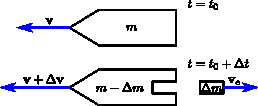
\includegraphics[width=0.6\linewidth]{figures/ciolkovszky.pdf}
    \caption{\centering A rakéta sebességének megváltozása a lendületmegmaradás törvényéből következik.}
    \label{fig:ciolkovszky}
\end{figure}

Írjuk fel a lendületmegmaradás törvényét. A rakétában ülők a gázt $\vec{v_e}$ sebességgel látják eltávozni. Kezdetben ($t = t_0$) a rendszer impulzusa $\vec{I}_0 = m\vec{v}$, $\Delta t$ idő elteltével a rendszer lendülete:
$\vec{I}_1 =(m - \Delta m)(\vec{v} + \Delta \vec{v}) + \Delta m \vec{v}_h$, azaz az \ref{eq:lenduletmegmaradas}. egyenlet alapján:
\begin{equation*}
  m\vec{v} = (m - \Delta m)(\vec{v} + \Delta \vec{v}) + \Delta m (\vec{v}-\vec{v_e})
\end{equation*}
\begin{equation*}
  m\vec{v} = m\vec{v} + m\Delta\vec{v} - \Delta m \vec{v} - \Delta m \Delta \vec{v} + \Delta m\vec{v} - \Delta m \vec{v_e}
\end{equation*}
A másodrendűen kicsi $\Delta m \Delta \vec{v}$ tagot elhanyagolhatónak tekinthetjük.
\begin{equation}
    m\Delta\vec{v} = \Delta m \vec{v_e}
    \label{eq:mdv-eq-dmve}
\end{equation}
Fejezzük be a levezetést. Tételezzük fel, hogy a környezetünk és a rakéta ideális, és nem hat semmilyen külső erő a rakétánkra. Mivel pozitív $\Delta m$ tömeget lövelünk ki, ezért a rakéta tömege az időben csökkeni fog, ezért legyen $\dd{m} = - \Delta m$.
\[-\dd{v} = v_e\frac{\dd{m}}{m}\]
Integráljunk. Jelölje a rakéta kezdeti tömegét $m_0$, üzemanyagnélküli tömegét pedig jelölje $m_{sz}$.
\[-\int_v^{v+\Delta v} \dd{v} = v_e \int_{m_0}^{m_{sz}} \frac{\dd{m}}{m}\]
\[-(v + \Delta v - v) = v_e\left(\ln{m_{sz}} - \ln m_0\right) \] 
\[\Delta v = v_e(\ln m_0 - \ln m_{sz})\]
\begin{equation}
    \Delta v = v_e\ln{\dfrac{m_0}{m_{sz}}}
\end{equation}
Ez az ideális rakéta egyenlet, amelyet Ciolkovszkij-egyenletnek is neveznek. Ez az egyenlet megmutatja, hogy egy ideális $m_0$ kezdeti és $m_{sz}$ végtömegű rakéta (üzemanyag tömege: $m_u = m_0 - m_{sz}$) és
$v_e$ a rakétát elhagyó gázsugár sebessége mellett mekkora sebességváltoztatásra képes a rakéta.

\subsubsection{A rakéta egyenlet nehézségi erővel és közegellenállással}

Sajnos a mi szimulációnkban hat külső erő, névlegesen a nehézségi erő és a közegellenállás, így ennek tudatában kell módosítanunk a levezetésen.
Alakítsuk át $\vec{F_t}$ erővé a gázsugár távozása által keltett lendületmegváltozást a rakétában. Newton II. törvénye alapján:
\begin{equation}
    \vec{F} = \dfrac{\Delta \vec{I}}{\Delta t} = m\dfrac{\Delta \vec{v}}{\Delta t}
    \label{eq:newton2}
\end{equation}
Esetünkben akkor az $\vec{F_t}$ erő levezethető a \ref{eq:mdv-eq-dmve}. egyenletből:
\[m\Delta\vec{v} = \Delta m \vec{v_e}\]
Osszunk $\Delta t$-vel:
\[m\dfrac{\Delta \vec{v}}{\Delta t} = \dfrac{\Delta m}{\Delta t} \vec{v_e}\]
Vezessük be az $\dot{m} = \dfrac{\Delta m}{\Delta t}$ kilépő tömegáramot. Ez azt mutatja meg, hogy időegységenként mekkora tömeg hagyja el a rakétát. Newton II. törvénye alapján pedig akkor ezek szerint:
\begin{equation}
    \vec{F_t} = -\dot{m}\vec{v_e}
\end{equation}

Vizsgáljuk a többi erőt is. A nehézségi erő a magasság és a tömegfüggvényében is változik. A rakétánkat a Földről indítjuk tengerszinten, a Föld
tömegközéppontjától $R_E = \qty{6,378}{km}$ magasságról. A Newton-féle gravitációs erő:
\begin{equation}
    F_{g} = \gamma \frac{Mm}{r^2}
\end{equation}
ahol $m$ és $M$ a két test tömege, $r$ pedig a középpontjaik távolsága. Esetünkben akkor a gravitációs erő a $h$ felszíntől mért magasság és az $m$ rakéta tömeg függvényében:
\begin{equation}
    F_g(m,h) = \gamma M \frac{m}{(R_E + h)^2}
    \label{eq:F_g-m-t}
\end{equation}

Most vizsgáljuk a közegellenállás erejét. Képlet alapján a közegellenállás:
\begin{equation}
    \vec{F_k} = - k\frac{1}{2}A\varrho\vec{v}^2
    \label{eq:kozegellenallas}
\end{equation}
ahol $k$ az alaki tényező, $A$ a test homlokfelülete (az a felület amely merőleges $\vec{v}$-re), $\varrho$ pedig a levegő sűrűsége. Modellezzük most a levehő sűrűségének
magasság függését a barometrikus egyenlettel:
\begin{equation}
    \varrho = \varrho_0 e^{-\frac{gh}{RT}}
\end{equation}
ahol $\varrho_0$ a tengerszinten lévő légnyomás, $R$ az univerzális gázállandó, $T$ pedig az itt állandónak tekintett hőmérséklet. Legyen $H = \frac{RT}{g} \approx \qty{8,4}{km}$ az ún. skálamagasság.
Így a barometrikus egyenlet:
\begin{equation}
    \varrho(h) = \varrho_0 e^{-h/H}
\end{equation}
Helyettesítsük ezt be a közegellenállást leíró \ref{eq:kozegellenallas}. egyenletbe.
\begin{equation}
    \vec{F_k}(h,\vec{v}) = - k\frac{1}{2}A\varrho_0 e^{-h/H}\vec{v}^2
\end{equation}

Összesítve tehát a rakátára ható eredő erő:
\begin{equation*}
    F = F_t - F_g - F_k
\end{equation*}
\begin{equation}
    F(m,\,h,\,v) = \dot{m}v_e - \gamma M_F\dfrac{m}{(R_E + h)^2} - k\frac{1}{2}A\varrho_0 e^{-h/H}v^2
\end{equation}

\subsection{A szimuláció leírása}
A szimulációt előretartó Euler módszerrel fogom megvalósítani. A diszkrét idejű szimulációnkban a sebesség a következő $k+1$-edik időpillanatban:
\[a[k] = \frac{F[k]}{m[k]} = \frac{\Delta v [k]}{\Delta t}\]
\[\Delta v[k] = \frac{F[k]}{m[k]}\Delta t\]
\begin{equation}
    v[k+1] = \frac{F[k]}{m[k]}\Delta t + v[k]
\end{equation}
A magasságra ugyanez:
\[v[k] = \frac{\Delta h[k]}{\Delta t}\]
\begin{equation}
    h[k+1] = v[k]\Delta t + h[k]
\end{equation}
És végül a tömeg:
\[-\dot{m} = \frac{\Delta m [k]}{\Delta t}\]
Azért kapott negatív előjelet, $\dot{m}$, mert negatív tömegváltozásról beszélünk.
\begin{equation}
    m[k+1] = m[k] - \dot{m}\Delta t
\end{equation}

% --------------------------------------------------    
% Irodalomjegyzék
% --------------------------------------------------
\newpage
\printbibliography

% --------------------------------------------------
% Függelék
% --------------------------------------------------

%\includepdf[pages=-]{contents/programkod.pdf} programkód beszúrása, ha szükséges

\end{document}
